\chapter{Sistema di autenticazione}


\section{Scopo del sistema}

Il sistema di autenticazione ha lo scopo di gestire le richieste di autenticazione da parte degli utenti e di fornire un token di sessione valido per l'accesso alle risorse protette.

\section{Descrizione del sistema}

Il sistema di autenticazione è definito da un microservizio che espone un'interfaccia REST per la gestione delle richieste di autenticazione degli utenti. Il microservizio è inoltre responsabile della generazione e della validazione dei token di sessione.

I token di sessione utilizzati sono del tipo JWT (JSON Web Token) e sono composti da tre parti separate da un punto. La prima parte contiene le informazioni relative all'algoritmo di hashing utilizzato per la firma del token, la seconda parte contiene le informazioni relative all'utente autenticato e la terza parte contiene la firma del token.

\section{Architettura del sistema}

Il sistema utilizza un'architettura esagonale, in cui il core del sistema si occupa della business logic ed offre:
\begin{itemize}
    \item Generazione dei JWT;
    \item Refresh dei JWT;
    \item Autenticazione degli utenti.
\end{itemize}

\begin{figure}[H]
    \centering
    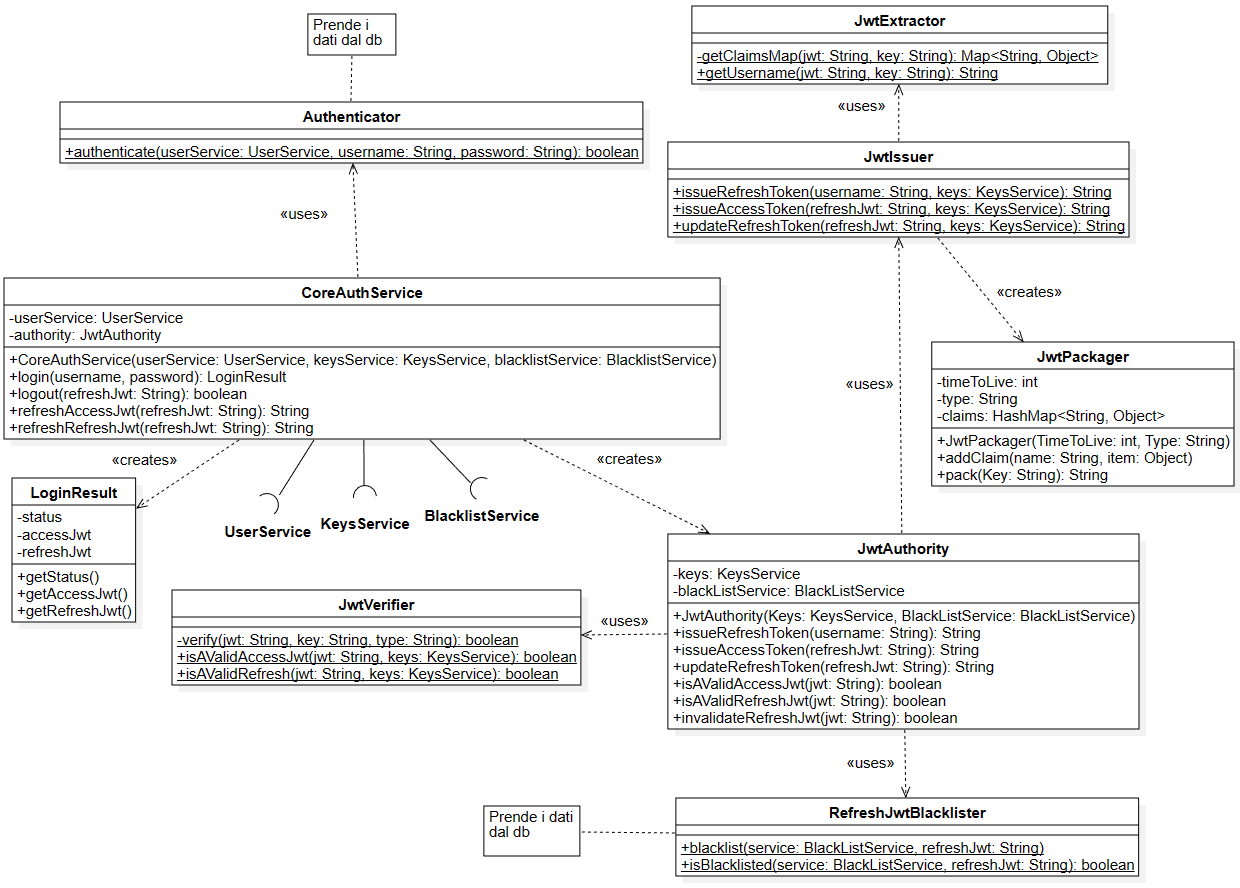
\includegraphics[width=\textwidth]{img/classi_auth.png}
    \caption{Diagramma delle classi del sistema di autenticazione}
\end{figure}

Il sistema offre poi un'interfaccia di tipo REST, e si connette sempre tramite l'utilizzo del sistema a porte ad un Database per la memorizzazione dei dati.

\subsection{I JWT}

Il sistema generale è pensato per utilizzare due tipologie di Token. Viene utilizzato un token di autorizzazione, che viene utilizzato per l'autenticazione e per l'accesso alle risorse protette degli altri microservizi e un token di refresh, che viene utilizzato per la generazione di un nuovo token di autorizzazione.

Ognuno dei microservizi del sistema accetta come valido un token generato da questo microservizio. Non accetterà però come valido un token di refresh.

Il token di refresh viene infatti riconosciuto solamente da questo sistema.

Il token di refresh ha durata di 2h, mentre il token di autorizzazione ha durata di 10 minuti.

\section{Interfaccia REST}

L'interfaccia rest viene esposta all'esterno e permette di effettuare le operazioni discusse nelle sotto-sezioni successive.

\subsection{Autenticazione}

POST /auth/login
